\chapter{Research Progress \& Results}
Following the previous section, this part is dedicated to reporting the progress of implementation by splitting into four stages of work.
The reasons behind the structure are to create consistent in the most relevant information without repeating the same topic.
They meant to create a proper way of describing the workflow and bring a better understanding of the task in hand.
They summarise findings and achievements upon expansion and modification based on discoveries and implementations in the future.
\begin{multicols}{2}
\begin{enumerate}
    \item \textit{Investigate}
    \item \textit{Integrating}
    \item \textit{Designing}
    \item \textit{Testing}
\end{enumerate}
\end{multicols}
Also, it aimed to present current findings and missing components that are left for investigation. \\
The Software Developer experience tells that to finish project successfully, it meant to be divided into Agile phases of development.
\subsection{Investigation}
This phase of the project may be considered as the most time-consuming and longest in development, as it does not contain any end goals that can be achieved by simple code implementation.
Throughout development, it reentered several phases of rethinking and rediscovering the process of very particular approaches.\\
There is no end to this section as it gets updated with every discovery, observation and result.
It suffered from inevitable changes, and, as it provided some exciting discoveries.
Finally, it will be summarised in a subsection by each hardware and software component.
\subsubsection{$360\circ$ camera}
One of the parts for recreating the surrounding environment is a 360-degree camera on Figure~\ref{fig:camera} on the right. 
In this case, the Kodak PIXPRO SP360 became the only available option.
However, despite the product cost, it was discovered that it is suited more for casual or touristic usage, rather than a severe component for upfront research.
It allows setting the recording stream to 60 frames per second (fps) with a 4k resolution, which allows for achieving high accuracy on a resulting image.
However, such video stream scale brings specific software difficulties as it requires preprocessing due to the memory size of the output.
PIXPRO also contains a useful application, allowing the establishment of a connection between the computer and the camera using either WiFi or NFC, which completely resolves the issue with storage.
Resulted video streams allow investigation of a full surrounding range with a decent elevation angle.
To use the device for other applications \footnote{except the official one}, it provides an easily accessible link, within a local IP address.
\begin{equation*}
 http://172.16.0.254:9176/
\end{equation*}
\begin{wrapfigure}{r}{0.35\textwidth}
    \centering
    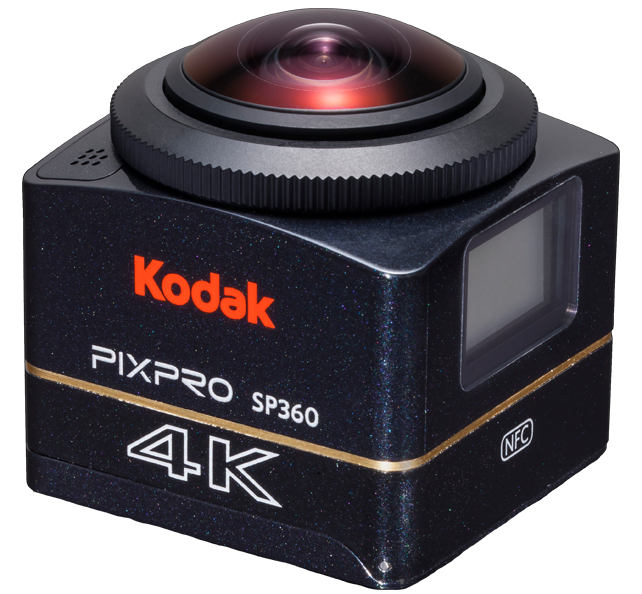
\includegraphics[width=0.30\textwidth]{project/images/camera.png}
    \caption{Kodak SP360}
    \label{fig:camera}
\end{wrapfigure}
Despite the high quality and good enough response speed, the drawback which the project met, is the format of the recording.
It talks about video output by format, which produced a hemisphere output. 
The problem with this stream is the actual usability.\\[1pc]
The Pixpro application setting does not allow the modification of the data stream upon recording.
The Unity Game engine supports dealing with a spherical or cubic texture. 
By providing it with only half of the image, the sphere got corrupted, and reconstructed video could barely consider as appropriate.\\[1pc]
An FFmpeg tool played its role very well in resolving this matter. 
However, by using an extra layer of configuration, video stream response gets slower, which requires sacrificing the quality of video in general. \\
The problem has resolved itself with some effort and video manipulation, but that was not the only one.\\[1pc]
The second issue is more problematic than simple software manipulation.
The PIXPRO application did not provide any means for changing settings. 
It served only as a trigger to start the recording process.\footnote{This particular issue was utterly ignored since the previous developer faced a similar problem.}
The best resolution to that is to replace the camera completely.
Some Raspberry Pi kits contain external cameras with a 360-degree view.
Maybe they can serve as a proper replacement.\\[1pc]
Originally, the camera was meant to serve both as a video stream and as a communication host between Unity, Tank and any other necessary components.
It turns out that additional devices \textbf{cannot} communicate with each other, over Camera WiFi hotspot. \\
The whole IP range is located within 172.16.1.* range, starting from 1 and 255(excluding 254). Such a weird configuration exists due to the way not to interfere with the actual video stream IP on location 254.
All credits to this discovery belong to \textit{nmap} network tool.
For only local usage, this tool was considered legitimate as there were no other alternatives.\\
The triggered issue, which required a total camera replacement, will be discussed later in Raspberry Pi subsection~\ref{subsec:RPI}.\\[1pc]
Finally, the delay between recording and actual reconstruction within a game is a separate matter to resolve.
The delay turned out to be significant since the video stream had to be modified and reapplied as textures following UDP protocol, instead of https, which will be discussed in Unity subsection~\ref{subsubsec:Unity}.
The previous argument ends up to be as another reason to replace this particular hardware with something more useful.
\subsubsection{Object Detection \& Machine Learning Nets}
The original idea of using a simple OpenCV library has proven to be quite useful in other similar kinds of projects, but not for this one, which takes much processing to care first.
It also showed good results after running some simple tests with a web camera to detect a specific object.
OpenCV has proven to be very good, in particular, to recognise the yellow colour as potential targets.
Initially, they were meant to look like small pong balls.
However, having something more powerful and experience in Machine Learning had to play itself more efficiently. \\[1pc]
During the general university study, outside of research time, there were several tasks in hand that required a certain degree of machine learning usage, TensorFlow in particular.
With the help of researchers and Lecturers, knowledge gained from their expertise becomes a significant contribution towards building a new efficient Neural Network to recognise tanks in the 360-degree image.
It is a good thing that through serving through the World Web, there were several libraries that provided a good example and API to use TensorFlow inside Unity with C\# Language.
However, all similar projects described earlier used only the CPU level to perform calculations, which does not give the best result of processing.
Luckily, Unity is aimed to use Computer Graphics, which means the next stage of learning with use NVIDIA CUDA libraries.
So far, all detections performed well on a Linux environment, which gave higher results than Windows, but those details and how CUDA with GPU may enhance this process are meant to be investigated by other researchers.
\subsubsection{Unity Game Engine} \label{subsubsec:Unity}
\begin{wrapfigure}{r}{0.3\textwidth}
    \centering
    
\includegraphics[width=0.25\textwidth]{project/images/Unity-Logo.png}
\end{wrapfigure}
Unity is an environment based on Game Engine, which is occasionally used for simulations and testing in some companies.
As a foundation and first-hand experience, the VRES project of Kitchen Assistant (EvKA) served as a starting point.
It was also meant to be deployed in Virtual Reality (VR) with the help of some gear.
Using similar techniques may simplify the overall integration. \\[1pc]
Most of the video games implemented so far require the usage of the keyboard, mouse, joystick or similar tools.
All of them, most of the time, required the usage of hands and fingers.
VR with different hand gear allows people to perform more actions, including some physical work.
Unity in this project will be the base, where all discoveries will come up as one end-up product.
All other details of how it turned out with implementation are discussed further down.
\subsubsection{VR Gear Set}
This section is the least investigated part, even if considered as the main topic of the project.
However, the reason behind such a lack of attempts is the final goal.
HTC Vive designed for smooth integration with Unity, using SteamVR as a base for development.
Their usage, limitations and type of suitable device will be acknowledged later.
\subsubsection{Raspberry Pi} \label{subsec:RPI}
\begin{wrapfigure}{r}{0.45\textwidth}
	\begin{center}
		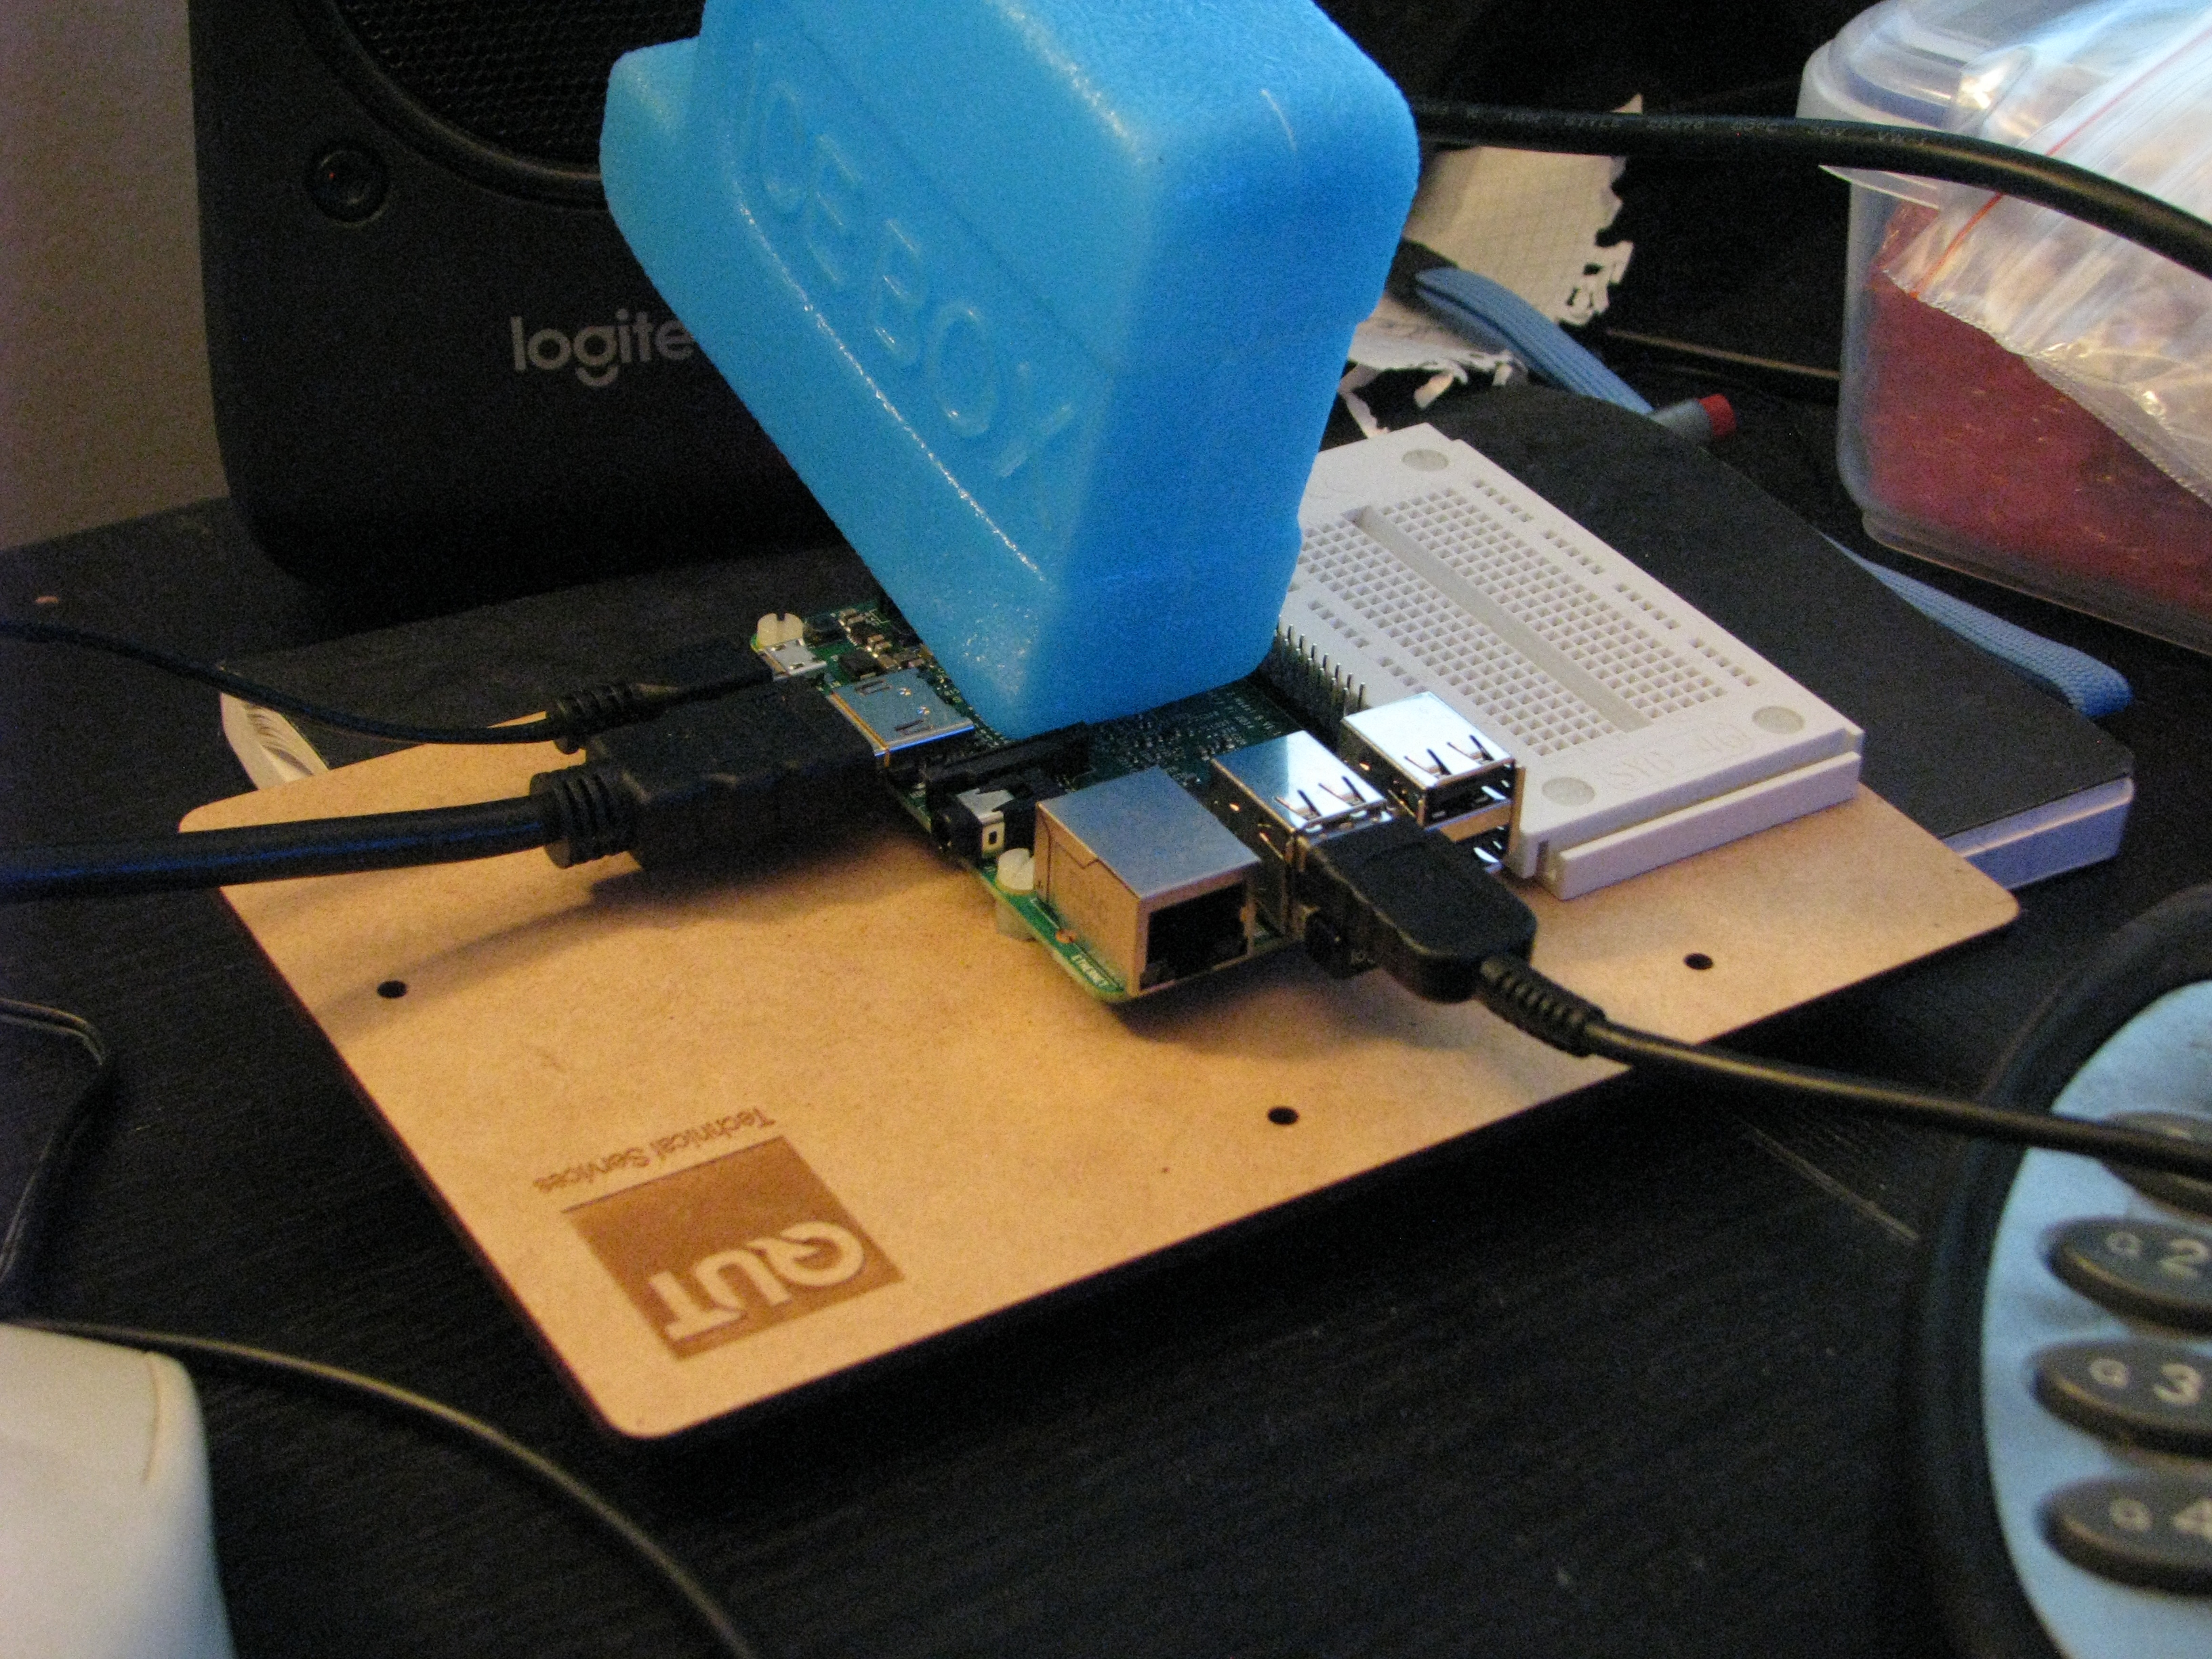
\includegraphics[width=0.35\textwidth]{project/images/IMG_1194.JPG}
	\end{center}
	\caption{Raspberry Pi cooling way}
	\label{fig:RPI}
\end{wrapfigure}
Another addition to the project and overall learning, in general, is an introduction to a new component - the controller of the tank itself. 
As a reminder, the current project builds on top of someone else's work, who constructed an actual voice-controlled tank. 
The way to send commands and drive this toy was performed using Raspberry Pi V3.
This particular version supports Wireless Communication.
R-Pi can establish a connection to a predefined WiFi hotspot and establish remote communication over either SSH or VNC. 
The Unity project will connect with Tank control over SPB, which allows mirroring all activities performed in Unity with the actual toy.
The concept of communication, package exchange or message way is used with socket communication.
By opening a socket server on Raspberry Pi through an IP address and port, Unity connects to the controller as a client and starts exchanging messages.
Through that talk, Tank will know what action is required to perform.
C\# and Python, the best message exchange package is ZMQ, after several hours of trials with different Libraries.
It is much simpler and more flexible than an ordinary socket.
The drawback of using R-Pi is the cooling system.
This particular model had to fan in the first place, that is why cooling was performed with whatever means possible, Figure~\ref{fig:RPI}.\\
Finally, Raspberry Pi contains a small circuit output - General Practice Input/Output (GPIO) pins.
They will be used to create an elementary testing circuit with LEDs on a breadboard, presented in the same Figure next to the controller.
\subsection{Integration}
The current phase of the project considers itself as the most programming-heavy one.
In the best case, it will focus on integrating all the parts in one C\# language-based environment.
In the worst case~\footnote{as, it became already}; it may become combinations of Python, C\# and bash.
However, the first workable results are present here.\\[1pc]
The goal is to adapt whatever discovery to the hardware in hand and integrate it with the Game Engine.
So far, only camera usage and object detection can provide reliable results.
By the end of the project, all other parts will have something more efficient to present.
\subsubsection{$360\circ$ camera}
There are several ways of using this IP address in Unity Advantage.
The investigation part comes with three modes, Skybox, around a box and a sphere.\\
The first method may sound tempting but far from the overall goal.
The whole sky becomes one large video file.
It is hardly a solution to the current problem. \\
Using Unity Extension called \textit{EasyMovieTexture}, the integration video stream with an object was a success.
Output different angles on a square frame allowed to produce five areas with video files shown during the play-through. \\
A sphere one using a similar extension had better results.
It can both accept a video stream or prerecorded file; the images and demos are located in further sections.
\subsubsection{Object Detection \& Machine Learning Nets}
OpenCV integration and colour detection were only the first step.
A TensorFlow plugin allows to integration of more complicated calculations into the project, for example, performing real-time detection, 
An easy and straightforward Mobile Net model already presented out of the box.
It helps to classify various objects from its' databases.
After performing certain pretraining with more tank-based data, it should be able to detect enemies, potential targets or other objects of interest.
The table in Appendix~\ref{fig:keras} represents official model benchmarks from Keras website~\cite{noauthor_applications_2018}.
Speed is a primary criterion for this project, which is why mobile net or other similar branches are going to be a priority in implementation.
\subsubsection{Unity Game Engine}
After completing and testing the first part of the planned work over the initial stages of the report, it was decided to move the project into a new version of Unity.
The entire project was rebuilding from the start using version 2018.3.1f1 and will remain the same until the end.
As a result, some of the assets required reimporting and some additional configured:
\begin{enumerate}
    \item \textbf{Ground Texture Pack:} To give surrounding area proper look.
    \item \textbf{T34 Tank Model:} A first testing Tank model.
    \item \textbf{QUT Tank Model:} Prefab, developed by Rodney Zsolczay.
    \item \textbf{Tileable Pack 01 (MAFUBASH):} An extra prefab
    \item \textbf{EasyMovieTexture V 3.69:} Upon moving to the new version and with new hardware, the older version appeared to be nonfunctional anymore.\footnote{Problems occurred around FFmpeg and AVformat library. Unfortunately, that was one of the issue updating to the latest version of Unity}
    \item \textbf{ML-Agents:} Plugin for using Machine Learning in Unity with Tensorflow-Csharp.
    \item \textbf{NetMQExample:} Used for socket communication with ZMQ Library
    \item \textbf{SteamVR:} Prefab used by HTC Vive to create a Virtual Reality Experience
\end{enumerate}
The next part will cover some of them in detail.
They are meant to bring clarity to the application and usage.
\begin{enumerate}
    \item \textbf{VR gear and SteamVR} \\
    HTC and Valve designed those tools for smooth integration with Unity.
    Their usage, limitations and type of suitable devices will be acknowledged later after presenting the first playable product.
    So far, SteamVR prefab and belonging documentation suited the overall project very well. 
    It caused no problem to apply it with HTC Vive, unlike PIXPRO in the section above. 
    The reason behind adding extra library support is manipulation with controllers. 
    The event system triggering has proven to be effective, though very different from every released version.
    It caused another development issue, which requires a separate and significant amount of time to study API.
    \item \textbf{EasyMovieTexture usage} \\
    It was an unfortunate coincidence that Version of Windows managed to update itself to latest without users notice, which lead to some incompatibility errors.\footnote{Take Away from this accident is -  NEVER work with Windows. 
    The next Unity project will work in a Linux environment. Even if it meant to use Wine HQ.} 
    The old version of the movie Texture had a significant issue upon running. 
    It may be relevant either to new hardware or new system configuration. 
    As a result, EasyMovieTeture required an update to the latest in order to support the UDP protocol stream received from FFmpeg.
    After that, usage of that prefab is only based on the given input and expected output.
    The streaming script is very adaptable and can be easily integrated into other components of the project.
    \item \textbf{FFmpeg AutoGen} \\
    The tool is designed to be integrated into Unity as a prefab, to use some of the Libraries with the power of Unity.
    It allows some simple video operation.
    However, this turned out to be not enough to discover a way to resolve the issue with the Video stream.
    In order to make changes, the library required manual recompilation.
    The effort and library management turned out to be too ineffective compared to how much it was spent with Tensorflow and from experience.
    Therefore FFmpeg was used outside of Unity to capture a video stream and to modify before entering Unity.
    The latest build from the official website provided all the necessary means.
    Details are followed in the Design section.
    \item \textbf{ML Agents} \\
    Machine Learning Agents Prefab was used to test first encounters with learned model usage.
    Some test scripts provided an excellent example of how to perform more complicated training, like balancing spheres, Figure~\ref{fig:ML-balancing} on a surface with varying gravity levels.
    The one which this project focuses on is Image recognition~\cite{unity-technologies_unity_2019}.
    It was designed to run on Android camera devices.
    However, using the TF-NetSharp library, it was a matter of time and skill to reapply learned configurations to the new environment. 
    As a result, with a trained Mobile Net model, Unity was able to recognise some of the surrounding objects.
    The next part will cover some of them in detail. 
    They are meant to bring clarity to the application and usage.
    \begin{figure}[H]
		\centering
		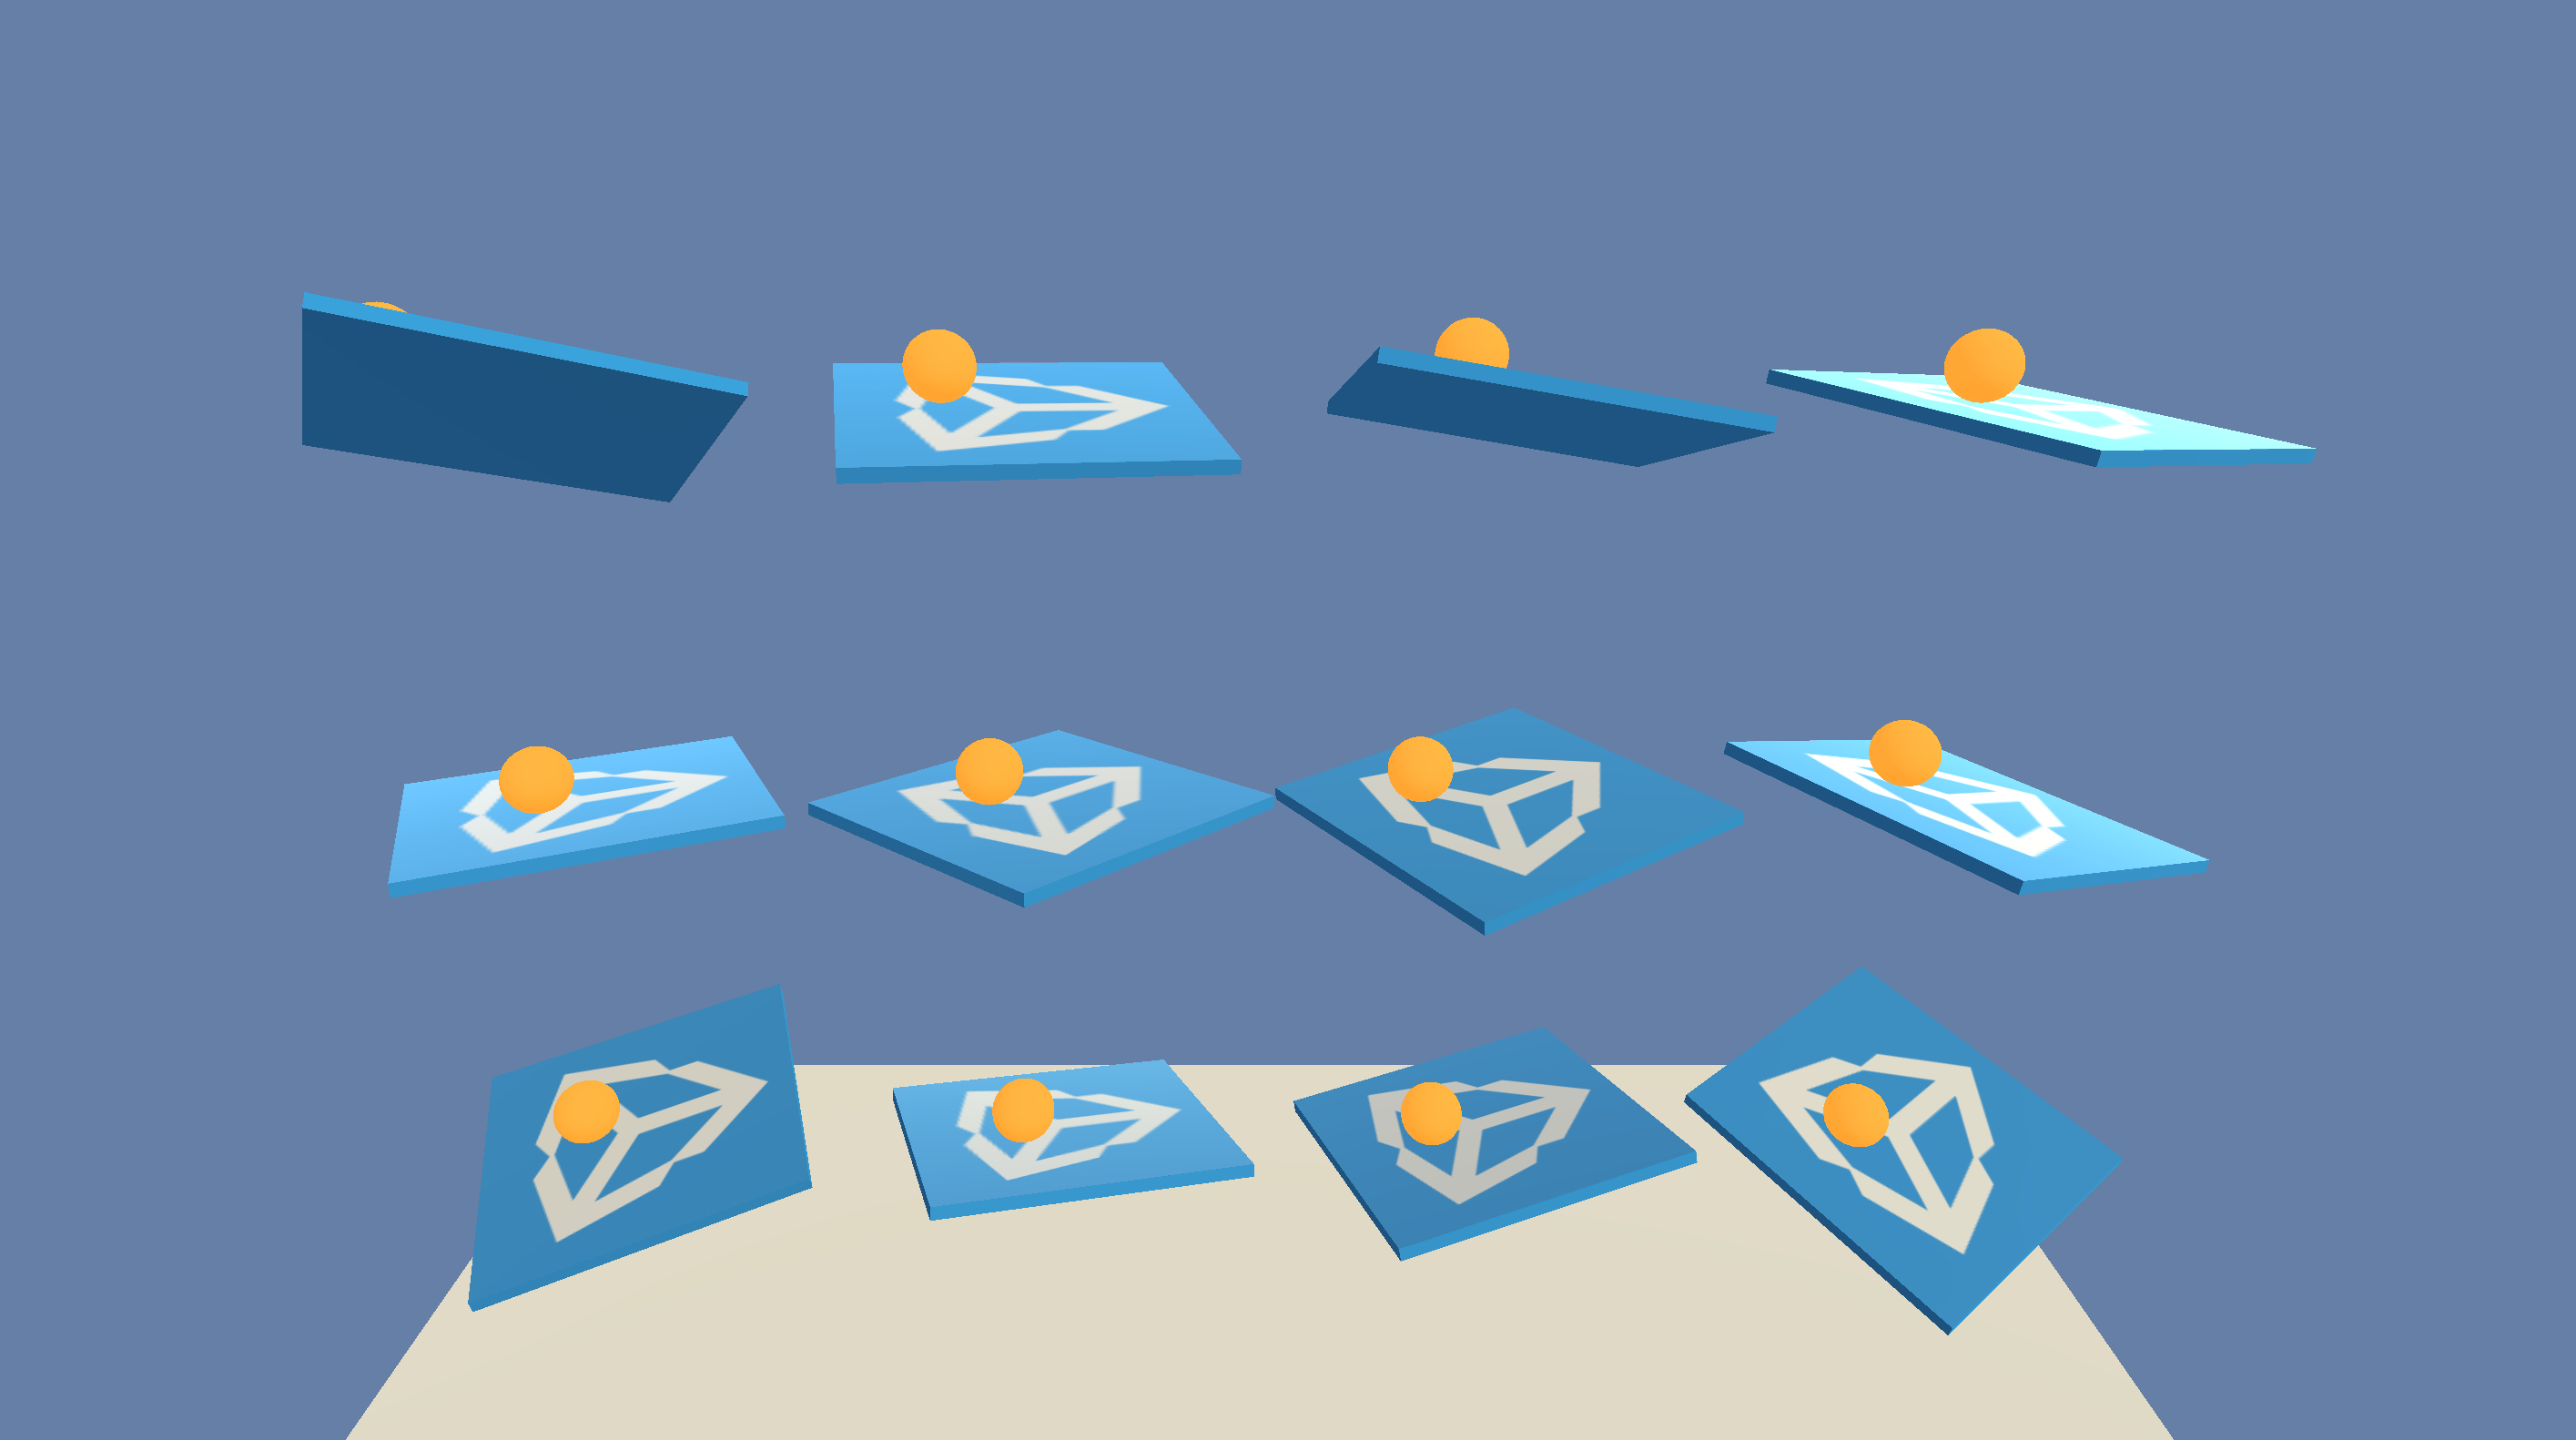
\includegraphics[width=0.5\linewidth]{project/images/balance.png}
		\caption{ML balancing example}
		\label{fig:ML-balancing}
	\end{figure}
\end{enumerate}
\subsection{Designing}
This phase of the project is the ground of all development.
Implementation results are meant to come up into one playable game, which is later used for testing.
\subsubsection{Unity Game Engine}
The testing area now consists of three primary things: a spherical object representing a 360 view, the ground floor of any type, and a simulated tank environment.
Using some basic knowledge from the Gaming Industry unit, the tank is now capable of moving by applying basic mechanics.\\
A sphere around the tank will simulate a real-world reality.
Top the tank contains another object, a sit for a player.
This location will be a placement for VR Glasses, where the Player controls the tank.
It represented as a VR camera view, which was provided by SteamVR prefab, with a place for controller events.
This environment is meant to simulate a real Mixed Reality experience using a headset and controllers.\\[1pc]
%The rest, regarding calculating distance, is simple math using cameras property. By detecting an object and placing hitting box around, it marks as a potential target. Shooting from a barrel will require some time to implement. \\
The process of integrating new features on top of the previous work went much smoother with updated versions of the components. 
If in the previous Unity was an entirely new environment for an Engineer, now, with the support of the supervisor and general practice with a Gaming Industry unit, project quality got improved.
The goal of the project remains the same, to present whatever discovery achieved during the investigation.\\[1pc]
In the future, the tester will have the possibility to manipulate with objects.
With interaction using controllers, the gamer must have all the means to move a tank inside the environment and, therefore, see how Unity will simulate precisely the same behaviour with the real tank.
Any manipulation will be recorded and sent back to the Engine for a 360-degree view.
FFmpeg Library and Machine Learning will be able to capture the stream and modify it with proper masking, marking enemy tanks.
With assistance from unity markers and barrel controllers, the player is meant to feel himself in a simulation of immersive experience - tank commander target practice, which will be detected by Unity and scored for every successful hit.
This kind of simulation is what project aims, and so far, it achieved significant progress.
\subsubsection{$360\circ$ camera}	
In the early stages of the project, camera reconstruction appeared as a square box around the player, as shown in subfigure~\ref{fig:oldLook}. 
Now, using an updated Movie texture plugin and modified stream, the entire surrounding is reconstructed over a hemisphere. 
A new look is represented on subfigure~\ref{fig:newLook}.
This section will cover the process in detail.\\
A square box did not provide a clear image over the surrounding area, and the way the video appeared on squares always changed itself with every run. 
That is why an example prefabs contained a spherical example too.
However, the tricky part was to reverse texture from the outside view, into inside.\\    
This operation is achieved by reversing a sphere shader.
It was a matter of trial and error to get a proper look, but a new Shader, which came from Unity documentation, has the following look in Appendix~\ref{apx:shader}. \\[1pc]
Another trial is cutting a sphere in half. 
The stream from a camera contained half the sphere output, which was directed within unity to cover the entire sphere.
Half of the image had to disappear, which caused a view loss.
One of the performed trials was to create an actual hemisphere object using a Blender 3D model, which was a success.
However, Applying a texture on top of that caused a similar loss.
Except for the wasted time, the idea brought no results.
\begin{figure}[H]
	\centering
	\begin{subfigure}[b]{0.4\textwidth}
		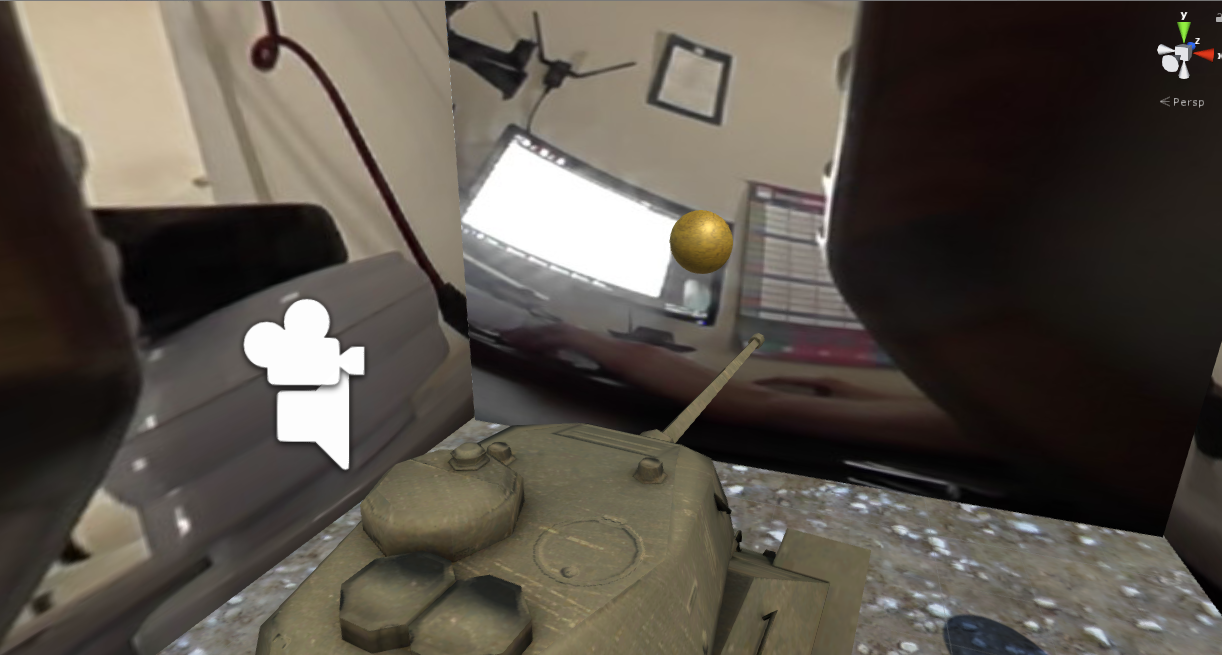
\includegraphics[width=\linewidth]{project/images/scene2.PNG}
		\caption{Old cube view}
		\label{fig:oldLook}
	\end{subfigure}	
	\begin{subfigure}[b]{0.24\textwidth}
		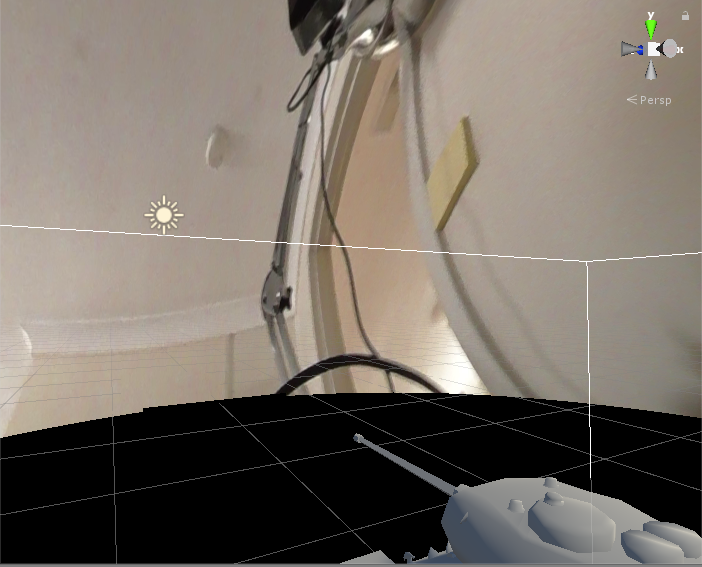
\includegraphics[width=\linewidth]{project/images/newLook1.PNG}
		\caption{New Spherical texture view}
		\label{fig:newLook}
	\end{subfigure}
	\caption{Images from Unity second usage}\label{fig:scene-developemt}
\end{figure}

\subsubsection{FFmpeg}
The most obvious approach, and the most successful one, was to modify a video stream with extra space and borders so that the relevant part of the video would appear as half of the sphere, the rest would be covered as a black area and will go beneath the Virtual view.
The Autogen version of FFmpeg inside Unity misses the following library: \textit{avformat-57}.
Directly copy/paste \textit{.dll} the file will not work out in this case.
Such operation requires recompilation of the entire build.
However, it was decided by the supervisor to use an independent build.\\
The FFmpeg with version 3.2 with the shared configuration~\cite{fate_ffmpeg_2018} build was able to capture the stream from the camera IP address \textit{(172.16.0.254:9176)} and modify with the following commands.
\begin{lstlisting}
    Input Command:
    ffmpeg -i http://172.16.0.254:9176/ -vf \
        "pad=width=2048:height=1024:x=512:y=0:color=black" \
        -vcodec mpeg4 -f mpegts udp://127.0.0.1:23001
    Siccesfull output:
        Stream #0:0: Video: mjpeg, yuvj422p(pc,bt470bg/
        unknown/unknown), 1024x1024, 25 tbr, 25 tbn, 25 tbc
\end{lstlisting}
Two boundary boxes are placed from both sides of a video stream so that they will fill the space at the bottom of the sphere. 
The following equation can describe the process of manual computing better:
\begin{align*}
    Given:\ H:1024,\ W:1024 \\
    PadSizeW&=W/2\ \&\ PadSizeH=\simeq (1-3) \\
    PadLocX1&=512 \ \&\ PadLocY1=0 \\
    PadLocX2&=W-512 \ \&\ PadLocY1=H \\
    ResultedVideoW&=W+2*(PadSizeW)=2048 \\
    ResultedVideoH&=H+2*(PadSizeH)=(1025-1034) \\
    Therefore: ResultedVideo\ H:(1025-1034),\ W:2048
\end{align*}
The address for access is presented below.
Using UDP protocol, Unity was able to capture that and produce the expected texture over the surroundings.
\begin{align*}
    udp://127.0.0.1:23001
\end{align*}
\textbf{Additional Commands which was used upon usage to concrete testing videos:}
\begin{lstlisting}
    list.txt:
        file '111_0001.MP4'
        file '111_0002.MP4'
        file '111_0003.MP4'
        file '111_0004.MP4'
    ----
    ffmpeg -safe 0 -f concat -i list.txt -c copy PreVideo.mp4
    ----
    ffmpeg.exe -i PreVideo.mp4 -vf \
        "pad=width=4320:height=2880:x=720:y=0:color=black" \
        -c copy output.mp4
\end{lstlisting}

\subsubsection{TensorFlow usage for ML}
%\textbf{Model integration into the thing. Seting up to .NET 4.6 Equivalent}
% File > Build Settings > Player Settings > Other Settings > Configuration > Scripting Runti
% Enable Tensorflow
The setup and usage of TensorFlow turned out to be much more complicated than it appeared initially.
The RTX2080Ti graphics cards have a new CUDA Compute capability level, which is not yet commonly used in primary TF libraries.  \\
\textit{Please consider a warning that if someone is planning to perform the installation, consider the following things:}
\begin{enumerate}
    \item Final build product may consume up to 15-20GB memory per compatibility support. 
The usage of RAM is very high and requires at least 6-8 GB; if this is not possible, consider the usage of flags, which will limit memory consumption.
    \item The process is very long, up to half an hour or more.\footnote{I managed to cook both lunch and dinner while the I7 overclocked processor was performing 6437 tasks in parallel with 12 threads.}
    \item Cease all activities before building.
    \item Installation process generally safe, as long as the machine is in working condition and keeps proper cooling effect\footnote{As a safety check, except for water cooling, compilation processed with three additional fans}.
\end{enumerate}
The next process will describe how the installation process went through:
\begin{multicols}{2}
\begin{enumerate}
    \item The steps for installation was taken from official Tensorflow website.\cite{tensorflow_build_2019}
    \item Python and setup environment configured with the help of Anaconda3. The separate environment used Python version 3.5. Any higher versions are not supported.        
    \item MSYS2 with the latest version had no issue in installation. It serves only as an environment for some Linux commands.
    \item GPU support required the following packages and their versions: 
    \begin{enumerate}
        \item CUDA 10.1
        \item cuDNN 7.4.2
        \item TensorRT 4.2
        \item Baze 0.19.2. WARNING! \footnote{Any younger or older version is unstable with Tensorflow. It was a matter of trials and error to get the appropriate one.} 
        \item XJN configuration is DISABLED
        \item AVX Support is ENABLED
    \end{enumerate}        
    \item Version of TF used for the build is 1.13r0
    \item Buidling Process was performed withn VS2015 x64 Native Tools CMD.
\end{enumerate}
\end{multicols}
The configuration and instructions above have to produce a proper wheel file, \".whl\" which is used to set up the Python PIP package manager. 
The command for building and installing is as follows:
\begin{lstlisting}
	Building with Bazel:
	bazel build --config=opt --define=no_tensorflow_py_deps=true
	            //tensorflow/tools/pip_package:build_pip_package
	
	Producing wl file:
	bazel-bin\tensorflow\tools\pip_package\build_pip_package
	            ../tensorflow-build/tensorflow_pkg

	Install wl file with PIP:
	pip install ..\tensorflow-build\tensorflow_pkg\
	            tensorflow-1.13.1-cp36-cp36m-win_amd64.whl
\end{lstlisting}
File path locations may vary depending on file structure. All work here is performed in the user home directory, with one folder:
\begin{lstlisting}
	C:/Users/User/Development/
\end{lstlisting}
As a result, GPU has shown incredible efficiency results in machine learning tasks. The whole procedure was worth it. \\
In the end, the small and efficient \textit{MobileNet} model was built to recognise all objects within the video stream.
The ml-agent prefab allowed to test the model and all remaining features of Unity itself.
The table with Keras benchmarks was moved to the Appendix~\ref{fig:keras}.
Benchmarks taken from Keras website~\cite{noauthor_applications_2018}.
\subsubsection{Socket communication}
Socket Communication was tested between Unity and Python within the same network.
ZMQ Library~\cite{omq_pyzmq_2019} has proven to be very useful for quick message exchange without additional configurations.
According to plans, Raspberry Pi will work as a server-side, then unity acts as a client and sends control commands in sequence. 
The server responds with results if it was successful or not, in case the tank gets stuck somewhere.
The testing was performed using TCP protocol under the following address.
\begin{equation}
    tcp://192.168.1.4:9999    
\end{equation}
Consider the usage of \textit{Nmap} tool for discovering which R-Pi has used IP address at initial connection.
\subsection{Testing}
Since the actual tank model was damaged and remained in a disassembled state, the project required other manners to test functionality.
\subsubsection{Testing Environment}
The Engineering Laboratory at QUT S block Level 9 had such a testing area for robotics students.
It is a small surrounding area with a field of 2 by 2 meters.
By printing a few images of the tank and sticking them to the walls or portable paper points, this testing area may create a sufficient environment.
The idea was to record a testing video with a 360-degree camera and move it manually around the testing area, as well as targets.
This way, at least some kind of action will be used within the simulation.\\[1pt]
\subsubsection{Simulating Tank Movement}
In order to test how the controller behaves with Unity, a small testing circuit with a straightforward Python script was developed within SPB.
Figure~\ref{fig:circuit} below represents a very simple circuit for Flashing LED upon calls through \textit{RPi.GPIO} Library.
Each LED represents one of the directions of the movement, if LED flashes, means tank successfully on the move.
At any point, the user, through console commands, is able to simulate an obstacle, informing that the tank has reached a limit of the arena and should not go any further.
\begin{figure}[H]
	\centering        
	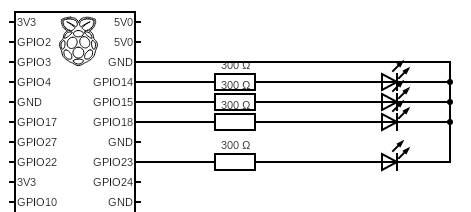
\includegraphics[width=0.75\textwidth]{project/images/circuit-cut.PNG}
	\caption{Testing LED circuit}
	\label{fig:circuit}
\end{figure}
\subsubsection{Results}
As a result, a prerecorded video, wirelessly connected Python controller, and HTC Gear create a reasonably reliable simulation within Unity Game Engine.
The recording of game functionality, ML detection and socket communication was demonstrated on video to the supervisor and will appear in the Final presentation. 
All Software details will be discussed in the next Prototype section. 
\subsection{Documentation of Development}
The final goal of everything is to bring usage for other users and researchers.
The aim is to set up proper instructions for every part which the project consists of.
So far, there is a Faster-RCNN architecture that was used to create models for Machine Learning.
The following link refers to Git Repository projects which are used over TensorFlow usage~\cite{smugglersmr_repository_2018}.\\
The document also consists of additional instructions for TensorFlow installation and FFmpeg manipulation, presented in this report above. 
The link to TF website\cite{tensorflow_build_2019}.
All non-relative code or script can be written by any low-level programmer.
However, they will still be appended to the Appendix for Reference.
\section{Prototype}
    After one year of research, implementation and trials with error, the game prototype ends up with following functionalities.
    Images below represent how the game scene went through a long process of changes to end up in a functional state.
	\begin{enumerate}
        \item Player First Person (FP) view through SteamVR prefab with the attached camera.
        \item Two HTCVive controllers, capable of providing simple user input.
        \item Tank object provided by PhD candidate, who supported research by providing a prefab of his Bachelor final year work. 
        \item Spherical texture, representing the movie scene, with the reversed shader.
        An object capable of output a proper 360 video stream inside the game.
        \item A canvas video appearing in front of the players view to summarise relevant information.
        \item Few spherical objects acted as markers for target detection.
    \end{enumerate}
	This project is a continuation from the researcher, who established a ground for a continuous video stream.
    Based on the result of his work, a 360degree camera video stream has been integrated before into the Unity game engine.
    His work used a sky-box environment build to create a realistic world. However, the current one relies on video conversion and streaming through \textit{MovieTexture}.
    To resolve the detection problem of the code with finding tanks and colours, it went through several implementations.
    The first implementation consisted of 5 out of 6 plates, surrounded tank from all directions, except the bottom, as shown in subfigure~\ref{fig:oldScene1}.
    Later, the environment got redeveloped into something more functional.
    As a result, a spherical object surrounded a player with only half of the size, creating a hemisphere.
	\begin{figure}[H]
		\centering
		\begin{subfigure}[b]{0.4\textwidth}
			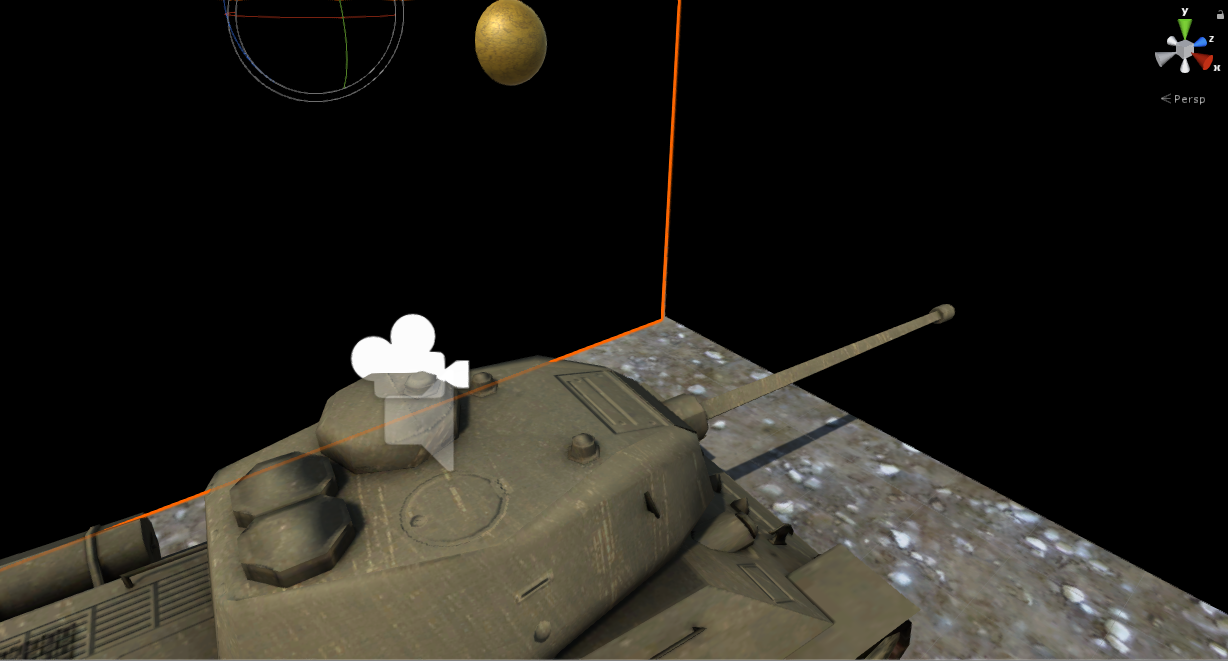
\includegraphics[width=\linewidth]{project/images/scene1.PNG}
			\caption{Changing view between tank and turret}
			\label{fig:oldScene1}
		\end{subfigure}
		\begin{subfigure}[b]{0.4\textwidth}
			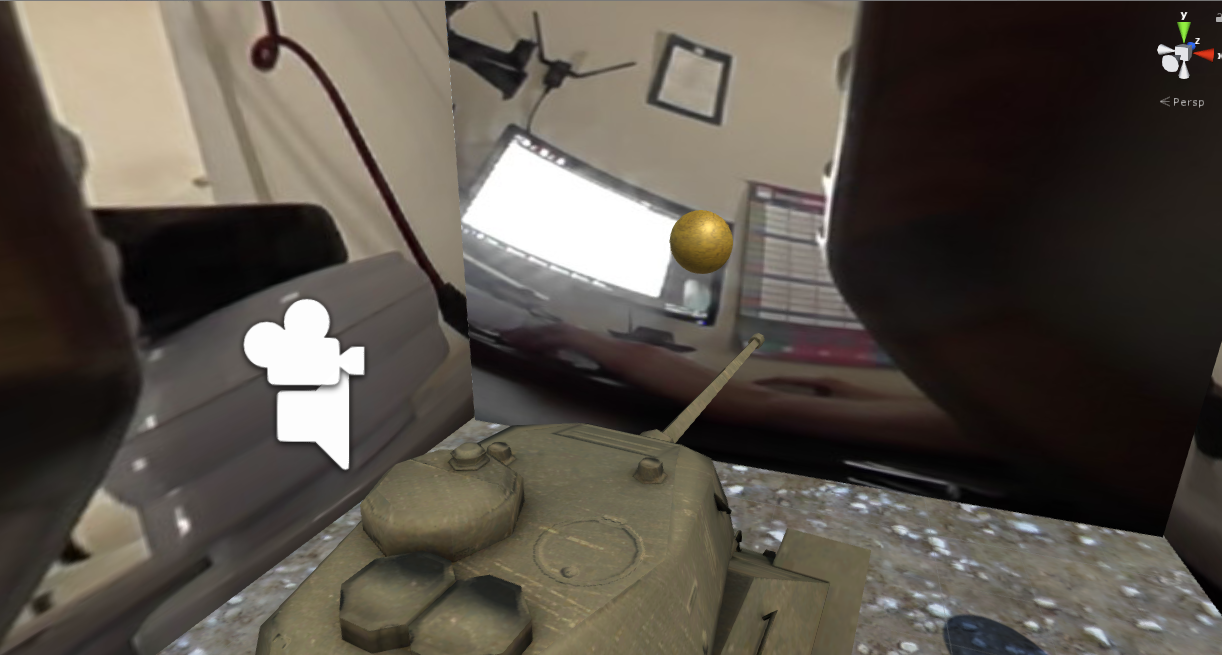
\includegraphics[width=\linewidth]{project/images/scene2.PNG}
			\caption{Entering Tank view screen}
			\label{fig:oldSscene2}
		\end{subfigure}
		\caption{Images from Unity base of development}\label{fig:scene-developemt}
	\end{figure}
	%%%%%%% Figure required reordering
	\begin{figure}[H]
    	\centering
    	\begin{subfigure}[b]{0.4\textwidth}
    		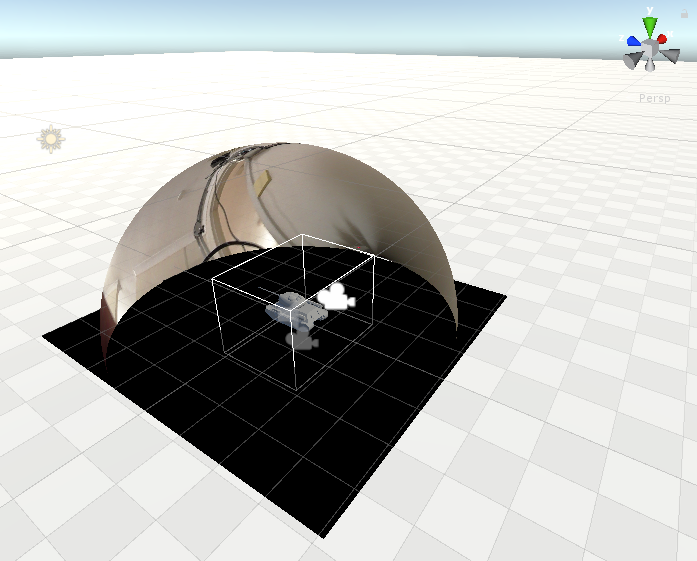
\includegraphics[width=\linewidth]{project/images/newLook2.PNG}
    		\caption{New representation of test area}
    		\label{fig:newScene1}
    	\end{subfigure}
    	\begin{subfigure}[b]{0.4\textwidth}
    		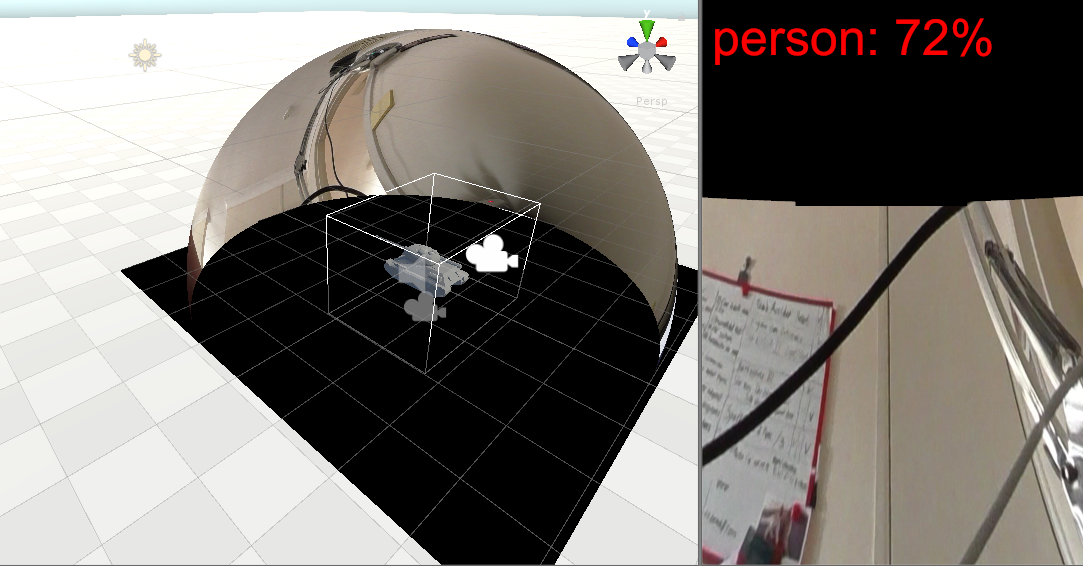
\includegraphics[width=\linewidth]{project/images/recognition.PNG}
    		\caption{Test Human recognition}
    		\label{fig:newScene2}
    	\end{subfigure}			
    	\caption{Images from Unity second base of usage}\label{fig:scene-developemt}
    \end{figure}
	As soon as the game starts, the texture produces the output of camera simulating realistic surrounding area.
    Subfigure~\ref{fig:newScene2} represents the programming area, which used for testing.
    OpenCV started detection, and as soon it finds potential yellow enough objects, a dark-yellow spherical object, which represents marker, gets moved to this location.
    A canvas video serves as a detection point, capable of determining with players view field has any potential targets and displays it in before of the user.
    At the same time, it places an invisible object in the environment, creating a hitbox for a player to aim. 
    This way game will be able to recognise if an enemy was hit through both in-game environments, and send information to the real-world testing area that enemy got destroyed.
    To calculate the distance from a camera to potential target objects and sum values with space in pixels from the tank to output plane, the article of QUT PhD candidate~\cite{sandino_estimation_nodate}, which provides sufficient information to implement the algorithm, is going to be used.
    Using the property of the camera, extracted from the documentation, it may give accurate enough results to perform the computation. \\[1pt]
    Originally, that idea purely relied on OpenCV and colour detection around player.
    However, through some cases like on subfigure~\ref{fig:oldSscene2} markers were moved to a completely wrong place, which most of the time requires manual adjustment.
    That is why the idea came up moving those detections to Machine Learning models.
    Using the support of GPU, such processes perform much faster and accurate. \\
%     Packages, which currently used by the projects are:
% 	%% Not all images present here yet.
% 	\begin{enumerate}
% 		\item EasyMovieTexture - used to create from texture movie screen
% 		\item Ground Texture Pack - to give surrounding area proper look
% 		\item ML-Agents - Plugin for using Machine Learning in Unity
% 		\item OpenCVUnity - Plugin for using OpenCV tools in scene
% 		\item T-34 - Model of the tank as point of work
% 	\end{enumerate}
	% Useless Figure
% 	\begin{figure}[H]
% 		\centering        
% 		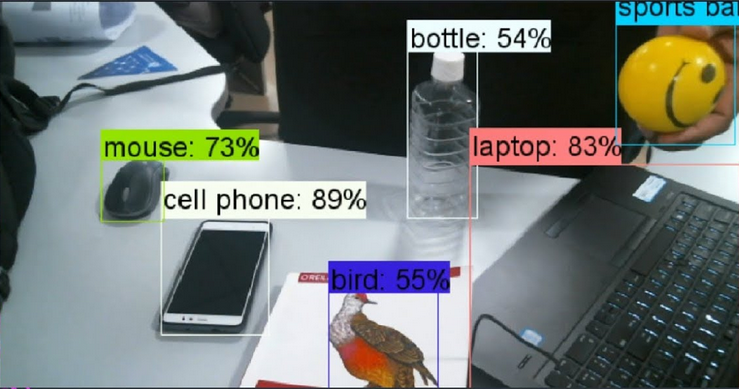
\includegraphics[width=0.5\textwidth]{project/images/ML-detec.png}
% 		\caption{Unity ML tutorial footage}
% 		\label{fig:mobile-neet}
% 	\end{figure}
%   As shown in Figure~\ref{fig:mobile-neet}. 
	With the help of material from different tutorials found over the web, it is possible to create a machine learning model for masking 
    However, it will be more efficient to use something more productive as Xception.
    In reality, this is the situation then speed matters more than accuracy.
    With QUT High-Performance Computer (HPC) Lyra, the training algorithm gets programmed for at least several days to build.
    As a result, only those, which produced maximum efficiency, were applied to report.
    The images above implements examples of~\cite{anuj_shah_tutorial_nodate} tutorial, with classifying several objects. For this case, only one will be enough.